%%%%%%%%%%%%%%%%%%%%%%%%%%%%% Define Article %%%%%%%%%%%%%%%%%%%%%%%%%%%%%%%%%%
\documentclass{article}
%%%%%%%%%%%%%%%%%%%%%%%%%%%%%%%%%%%%%%%%%%%%%%%%%%%%%%%%%%%%%%%%%%%%%%%%%%%%%%%

%%%%%%%%%%%%%%%%%%%%%%%%%%%%% Using Packages %%%%%%%%%%%%%%%%%%%%%%%%%%%%%%%%%%
\usepackage{ctex}
\usepackage{geometry}
\usepackage{graphicx}
\usepackage{pgfplots}
\usepackage{float}
\usepackage{minted}
\usepackage{hyperref}
\hypersetup{
    colorlinks=true,
    pdfstartview=Fit,
    pdfcreator={Shit},
    pdfproducer={Big shit}}
%\usepackage{amssymb}
%\usepackage{amsmath}
%\usepackage{amsthm}
%\usepackage{empheq}
%\usepackage{mdframed}
%\usepackage{booktabs}
%\usepackage{lipsum}
%\usepackage{color}
%\usepackage{psfrag}
%\usepackage{bm}
%%%%%%%%%%%%%%%%%%%%%%%%%%%%%%%%%%%%%%%%%%%%%%%%%%%%%%%%%%%%%%%%%%%%%%%%%%%%%%%

% Other Settings

%%%%%%%%%%%%%%%%%%%%%%%%%% Page Setting %%%%%%%%%%%%%%%%%%%%%%%%%%%%%%%%%%%%%%%
\geometry{a4paper}

%%%%%%%%%%%%%%%%%%%%%%%%%%%%%%% Plotting Settings %%%%%%%%%%%%%%%%%%%%%%%%%%%%%
%\usepgfplotslibrary{colorbrewer}
%\pgfplotsset{width=8cm,compat=1.18}
%%%%%%%%%%%%%%%%%%%%%%%%%%%%%%%%%%%%%%%%%%%%%%%%%%%%%%%%%%%%%%%%%%%%%%%%%%%%%%%

%%%%%%%%%%%%%%%%%%%%%%%%%%%%%%% Title & Author %%%%%%%%%%%%%%%%%%%%%%%%%%%%%%%%
\title{实验二: SPARK基础编程方法}
\author{胡嘉鑫 \and 102102145}
\date{\today}
%%%%%%%%%%%%%%%%%%%%%%%%%%%%%%%%%%%%%%%%%%%%%%%%%%%%%%%%%%%%%%%%%%%%%%%%%%%%%%%

\begin{document}
    \maketitle
    \tableofcontents

    \section{实验目的}
    \begin{itemize}
      \item	理解SPARK工作流程;
      \item	掌握SPARK基础编程方法.
    \end{itemize}

    \section{实验平台}
    \begin{itemize}
      \item OS: Linux
      \item Hadoop v3.1.3
      \item JDK v1.8
      \item Spark: 3.4.0
    \end{itemize}

    \section{实验步骤}

    \subsection{数据去重}

    \subsubsection{Problem Description}

    描述: 编写独立应用程序实现数据去重, 对于两个输入文件A和B, 编写Spark独立应用程序(推荐使用Scala语言),
    对两个文件进行合并,并剔除其中重复的内容,得到一个新的文件C。(文件A,B如下).

    Input(输入文件 A):

    \noindent 20170101 x \\
    20170102 y \\
    20170103 x \\
    20170104 y \\
    20170105 z \\
    20170106 z

    Input(输入文件 B):

    \noindent 20170101 y \\
    20170102 y \\
    20170103 x \\
    20170104 z \\
    20170105 y

    Expected output:

    \noindent 20170101 x \\
    20170101 y \\
    20170102 y \\
    20170103 x \\
    20170104 y \\
    20170104 z \\
    20170105 y \\
    20170105 z \\
    20170106 z

    \subsubsection{Code}

\begin{center}
\begin{minted}[xleftmargin=5mm]{scala}
package net.homework

import org.apache.spark.SparkConf
import org.apache.spark.SparkContext
import org.apache.spark.SparkContext._

import java.nio.file.Paths

object App {
  def main(args : Array[String]) : Unit = {
    val cwd = Paths.get("").toAbsolutePath.toString

    val inputPath = "file://" + cwd + "/input"
    val outputPath = "file://" + cwd + "/output"
    val inputFile0 = inputPath + "/A.txt"
    val inputFile1 = inputPath + "/B.txt"

    val conf = new SparkConf().setMaster("local").setAppName("pro1")
    val sc = new SparkContext(conf)

    val input0 = sc.textFile(inputFile0)
    val input1 = sc.textFile(inputFile1)

    val unionRes = input0.union(input1)

    val res = unionRes.distinct.sortBy(_.split(" ")(0))
    res.saveAsTextFile(outputPath)
  }
}
\end{minted}
\end{center}

    \subsubsection{Result}

    \begin{figure}[h]
      \begin{center}
        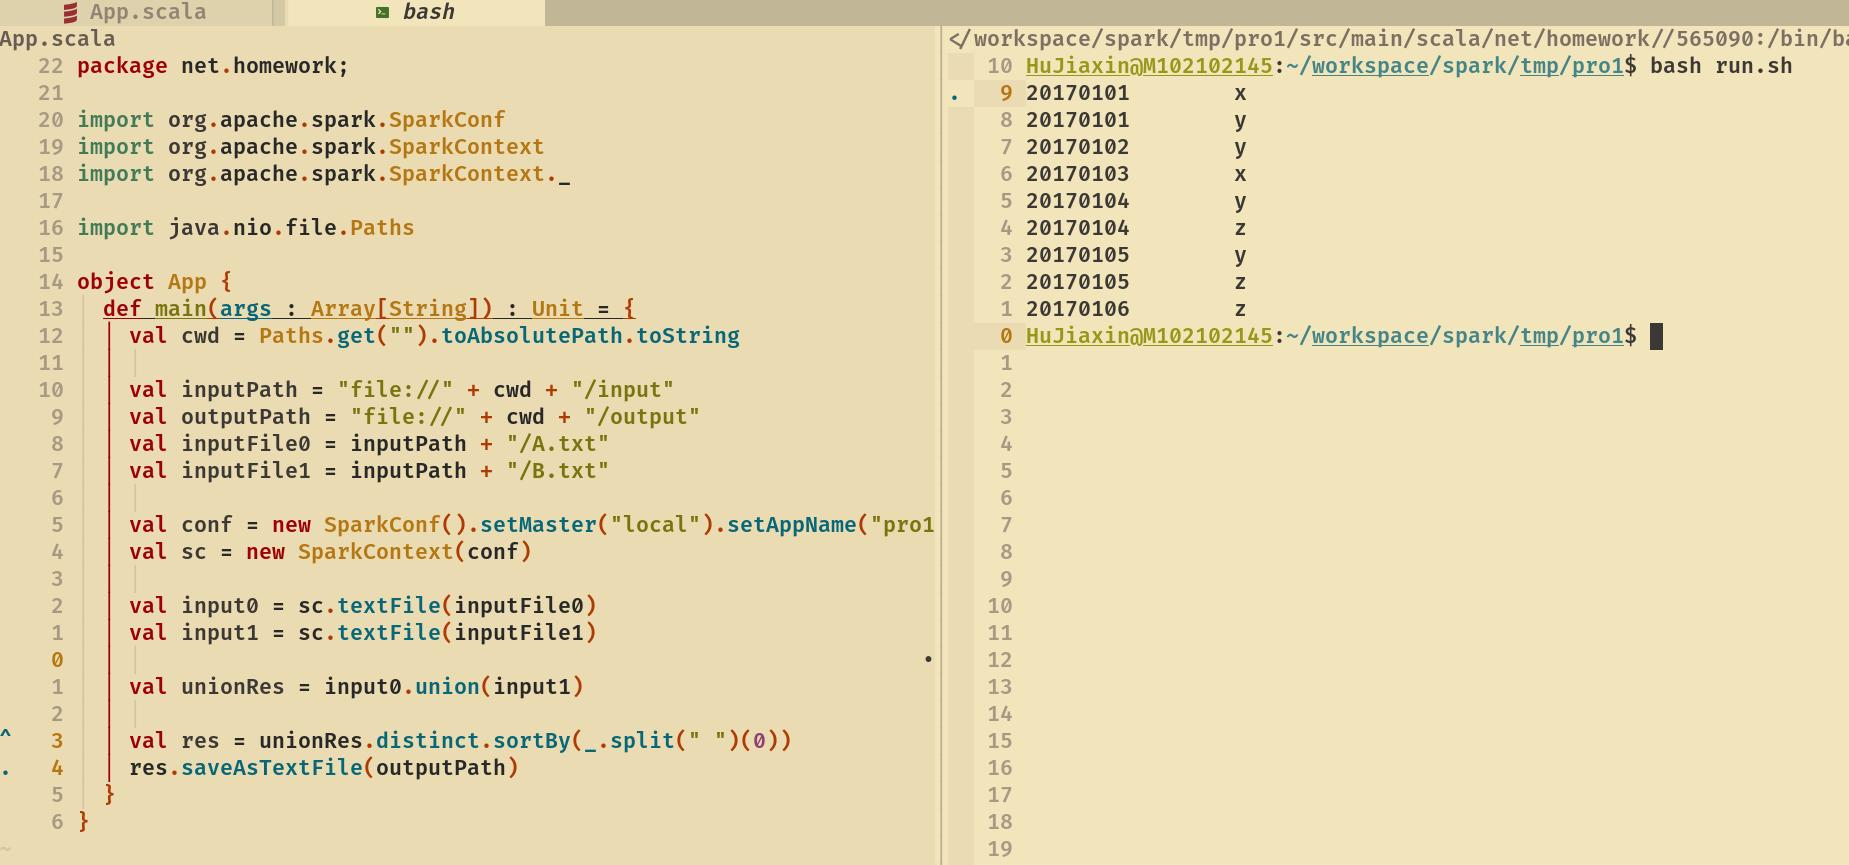
\includegraphics[width=0.95\textwidth]{./figures/1.jpg}
      \end{center}
      \caption{数据去重}
    \end{figure}


    \subsection{求平均值}

    \subsubsection{Problem Description}

    描述:每个输入文件表示班级学生某个学科的成绩,每行内仅由两个字段组成,第一个是学生名字,第二个是学生的成绩;
    编写Spark独立应用程序(推荐使用Scala语言)求出所有学生的平均成绩,并输入到一个新文件中。(各个科目的程序文件如下)

    Algorithm 成绩:

    \noindent 小明 92 \\
    小红 87 \\
    小新 82 \\
    小丽 90

    Database 成绩:

    \noindent 小明 95 \\
    小红 81 \\
    小新 89 \\
    小丽 85

    Python 成绩:

    \noindent 小明 82 \\
    小红 83 \\
    小新 94 \\
    小丽 91

    平均成绩如下:

    \noindent (小红,83.67) \\
    (小新,88.33) \\
    (小明,89.67) \\
    (小丽,88.67)

    \subsubsection{Code}

\begin{center}
\begin{minted}[xleftmargin=5mm]{scala}
package net.homework

import org.apache.spark.SparkConf
import org.apache.spark.SparkContext
import org.apache.spark.SparkContext._

import java.nio.file.Paths
import java.io.File

object App {
  def main(args : Array[String]) : Unit = {
    val cwd = Paths.get("").toAbsolutePath.toString

    val inputPath = "file://" + cwd + "/input"
    val outputPath = "file://" + cwd + "/output"

    val conf = new SparkConf().setMaster("local").setAppName("pro2")
    val sc = new SparkContext(conf)

    val textData = sc.wholeTextFiles(inputPath)
    val textContent = textData.map(_._2).flatMap(_.split("\n"))

    val dir = new File(s"${cwd}/input")
    var subjectCount : Double = 1
    if (dir.isDirectory) {
      subjectCount = dir.listFiles().count(_.isFile)
    }

    val res = textContent.map(
      x => (x.split("\t")(0), x.split("\t")(1).toInt)
    ).reduceByKey(
      (val1, val2) => val1 + val2
    ).map(
      x => (x._1, f"${x._2/subjectCount}%.2f")
    )

    res.saveAsTextFile(outputPath)
  }
}
\end{minted}
\end{center}

    \subsubsection{Result}

    \begin{figure}[H]
      \begin{center}
        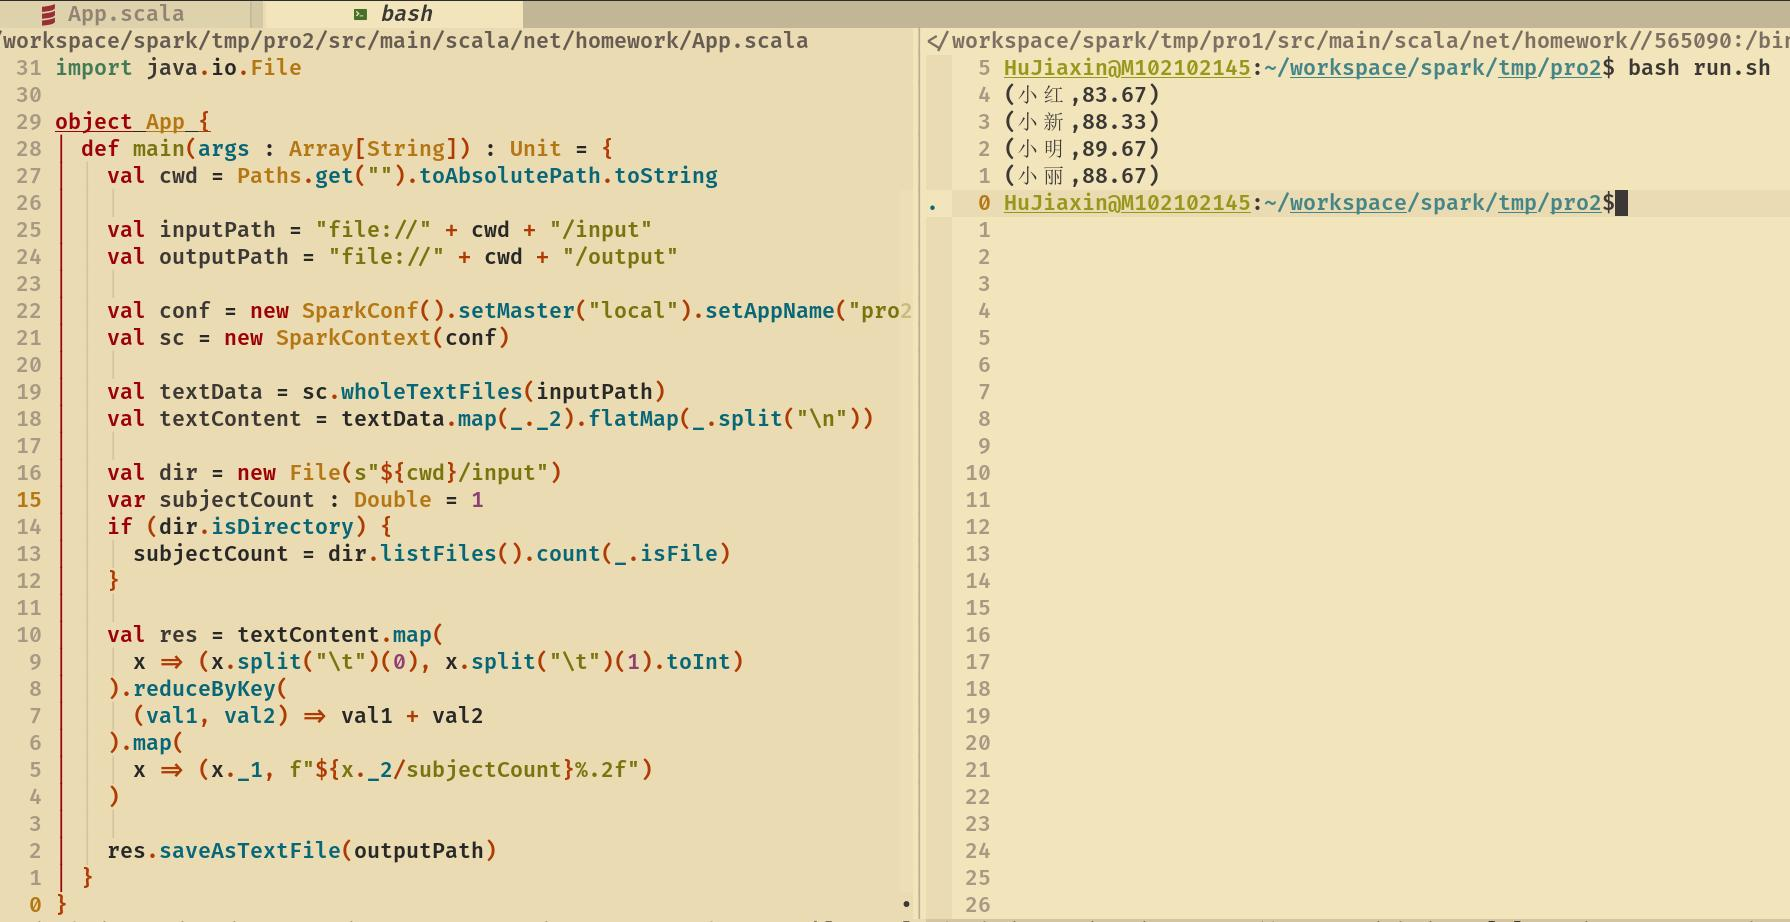
\includegraphics[width=0.95\textwidth]{./figures/2.jpg}
      \end{center}
      \caption{求平均值}
    \end{figure}

    \subsection{人数, 身高统计}

    \subsubsection{Problem Description}

    描述: 对于文件 people.txt, 该文件包含了序号、性别和身高三个列,
    编写Spark应用程序,计算得到
    男性总数、女性总数、男性最高身高、女性最高身高、男性最低身高、女性最低身高、男性平均升高、女性平均身高。

    文件形式如下:

    \noindent 0	F	168 \\
    1	F	141 \\
    2	M	184 \\
    3	F	186

    \subsubsection{Code}

\begin{center}
\begin{minted}[xleftmargin=5mm]{scala}
package net.homework

import org.apache.spark.SparkConf
import org.apache.spark.SparkContext
import org.apache.spark.SparkContext._

import java.nio.file.Paths
import java.io.File

object App {
  def main(args : Array[String]) : Unit = {
    val cwd = Paths.get("").toAbsolutePath.toString

    val inputPath = "file://" + cwd + "/input"

    val conf = new SparkConf().setMaster("local").setAppName("pro3")
    val sc = new SparkContext(conf)

    val textData = sc.wholeTextFiles(inputPath)
    val textContent = textData.map(_._2).flatMap(_.split("\n"))

    val people = textContent.map(
      x => {
        val arr = x.split("\t")
        (arr(2).toDouble, arr(1))
      }
    )

    val male = people.filter(x => x._2 == "M").map(_._1)
    val female = people.filter(x => x._2 == "F").map(_._1)

    val numOfMale = male.count
    val numOfFemale = female.count

    val maxHeightOfMale = male.max
    val maxHeightOfFemale = female.max

    val minHeightOfMale = male.min
    val minHeightOfFemale = female.min

    val avgHeightOfMale = male.reduce(
      (val1, val2) => val1 + val2
    ) / numOfMale
    val avgHeightOfFemale = female.reduce(
      (val1, val2) => val1 + val2
    ) / numOfFemale

    println(s"(男性总数, 女性总数): ($numOfMale, $numOfFemale)")
    println(s"(男性最高身高, 女性最高身高): ($maxHeightOfMale, $maxHeightOfFemale)")
    println(s"(男性最低身高, 女性最低身高): ($minHeightOfMale, $minHeightOfFemale)")
    println(s"(男性平均身高, 女性平均身高): ($avgHeightOfMale, $avgHeightOfFemale)")
  }
}
\end{minted}
\end{center}

    \subsubsection{Result}

    \begin{figure}[H]
      \begin{center}
        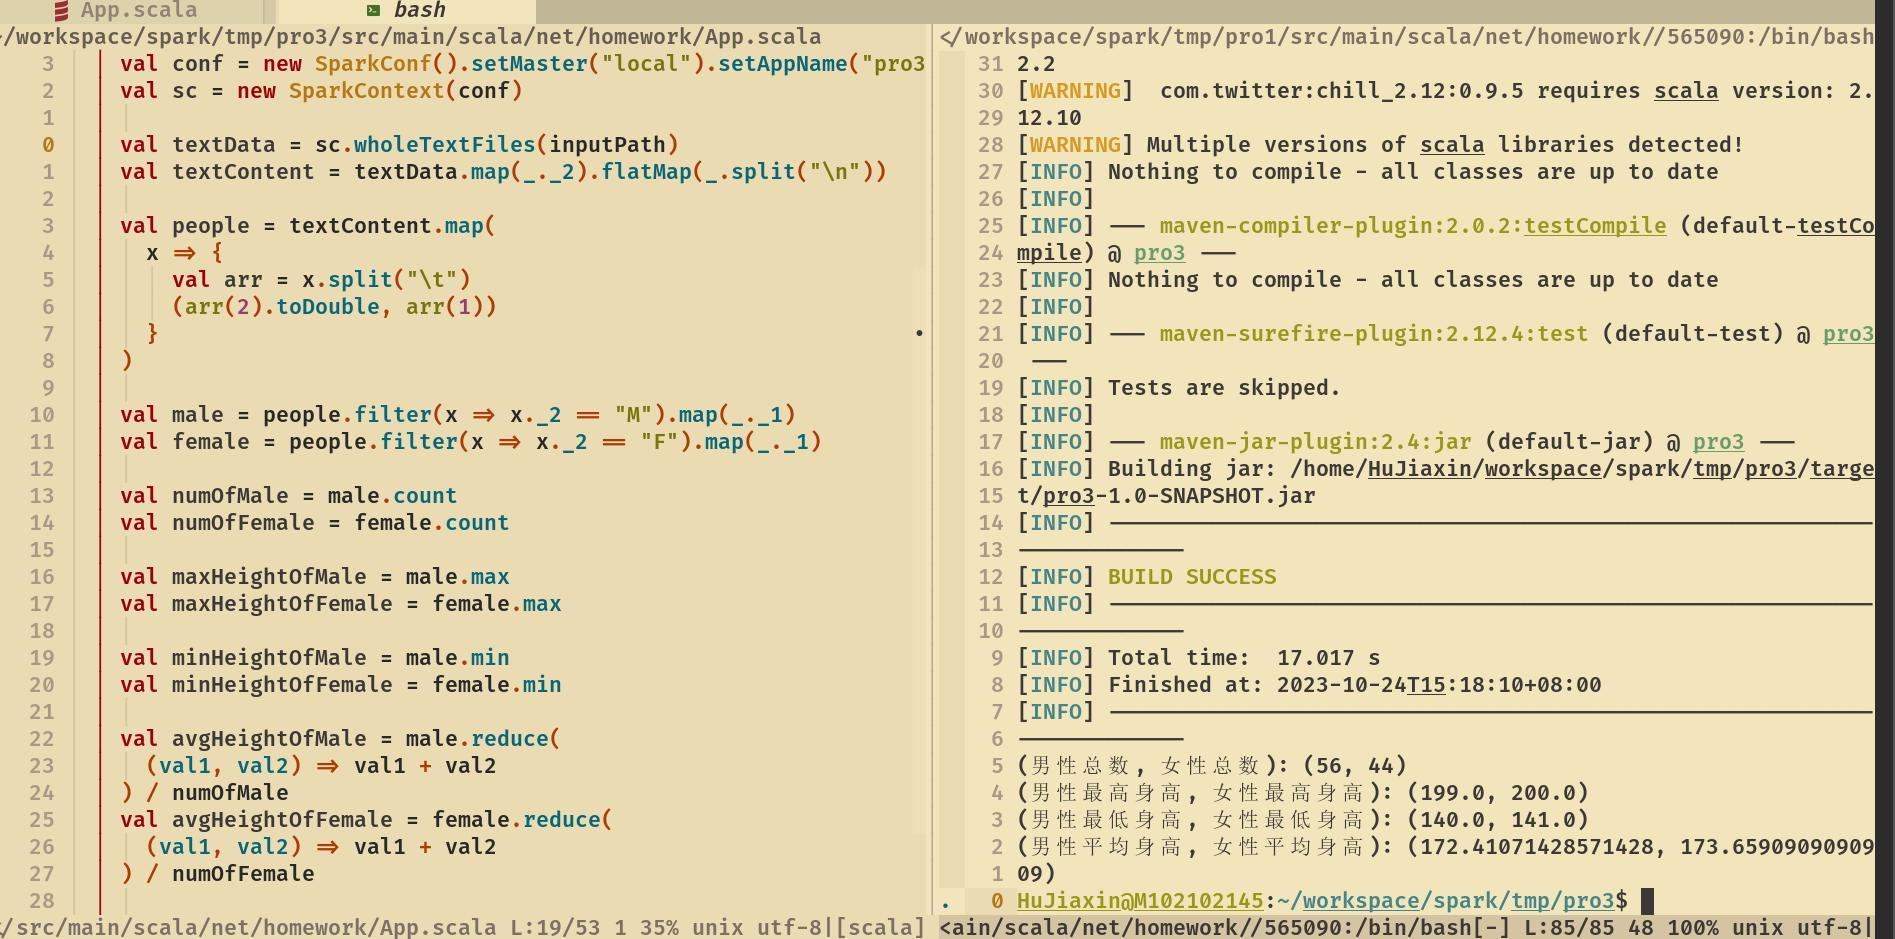
\includegraphics[width=0.95\textwidth]{./figures/3.jpg}
      \end{center}
      \caption{人数, 身高统计}
    \end{figure}

    \subsection{用户关系统计}

    \subsubsection{Problem Description}

    描述: 对于文件 relationship.txt,数据形式示例如下:A<B,C,D,F,E,O,表示用户B,C,D,F,E,O关注了A,
    现要求分别计算每个用户被关注的数量以及每个用户关注的数量。

    \subsubsection{Code}

\begin{center}
\begin{minted}[xleftmargin=5mm]{scala}
package net.homework

import org.apache.spark.SparkConf
import org.apache.spark.SparkContext
import org.apache.spark.SparkContext._

import java.nio.file.Paths

object App {
  def main(args : Array[String]) : Unit = {
    val cwd = Paths.get("").toAbsolutePath.toString

    val inputPath = "file://" + cwd + "/input"
    val outputPath = "file://" + cwd + "/output"

    val conf = new SparkConf().setMaster("local").setAppName("pro4")
    val sc = new SparkContext(conf)

    val textData = sc.wholeTextFiles(inputPath)
    val textContent = textData.map(_._2).flatMap(_.split("\n"))

    val res = textContent.map(
      x => {
        val arr = x.split("<")
        (arr(0), arr(1).split(","))
      }
    ).flatMap(
      x => {
        var ret = List((x._1, (x._2.length, 0)))
        for (fan <- x._2) {
          ret = (fan, (0, 1)) +: ret
        }
        ret
    }).reduceByKey(
      (val1, val2) => (val1._1 + val2._1, val1._2 + val2._2)
    ).map(
      x => (x._1, x._2._1, x._2._2)
    ).sortBy(_._1)

    res.saveAsTextFile(outputPath)
  }
}
\end{minted}
\end{center}

    \subsubsection{Result}

    \begin{figure}[H]
      \begin{center}
        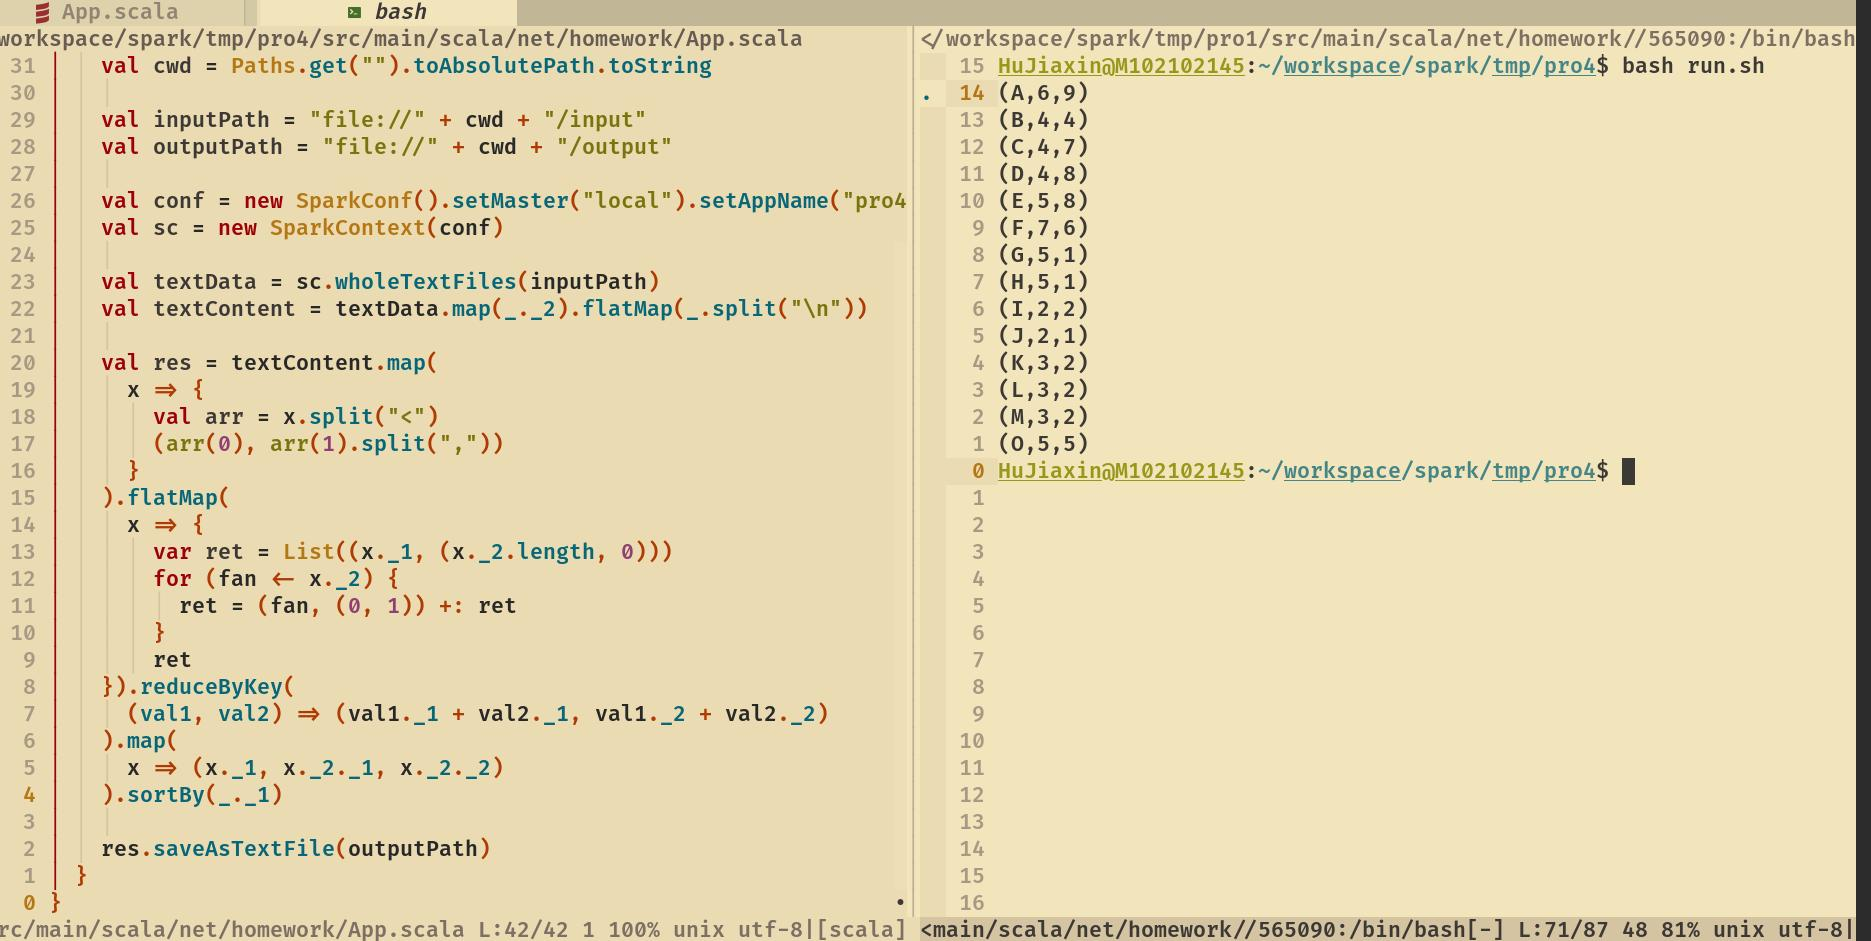
\includegraphics[width=0.95\textwidth]{./figures/4.jpg}
      \end{center}
      \caption{用户关系统计}
    \end{figure}

    \section{出现的问题及其解决方案}
    没有问题.
\end{document}
